\documentclass[12pt]{article}
\usepackage[margin=0.5in,paper=a4paper]{geometry} 
\usepackage[x11names]{xcolor}                     
\usepackage{tikz}
\usepackage{euler}       

\begin{document}
\thispagestyle{empty} 

\begin{center}
  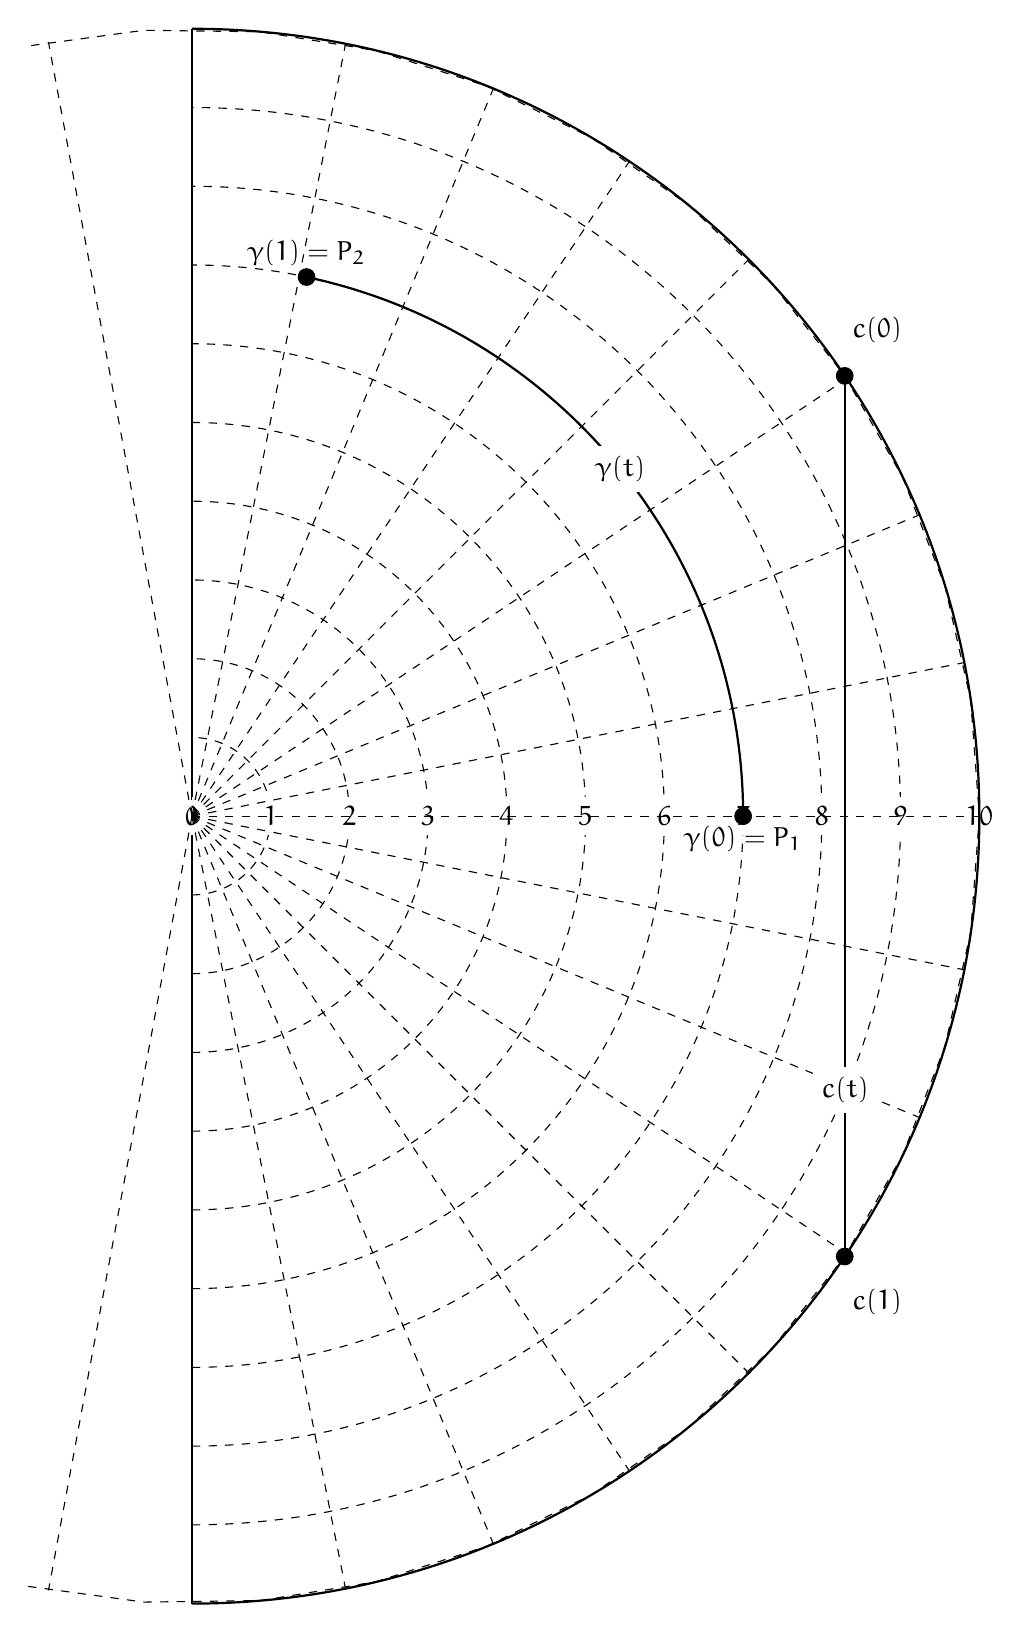
\begin{tikzpicture}
  \draw[black ,thick] (0,10)--(0,-10);
    %Circles 
    \foreach \r in {0,1, 2,...,9}
      \draw[rotate = 180 ,black, dashed] (0,\r) arc(90:270:\r)node[midway,fill=white]{$\r$};  
      \foreach \r in {10}
      \draw[rotate = 180 ,black, thick] (0,\r) arc(90:270:\r)node[midway]{$\r$}; 
     
      \foreach \a in {0,11.25,...,90}
      \draw[black,dashed] (\a:0) -- (\a:10); 
       \foreach \a in {281.25,292.5,...,359}
      \draw[black, dashed] (\a:0) -- (\a:10); 
       \draw [black,dashed,domain=-102:102] plot ({10*cos(\x)}, {10*sin(\x)});
      
\draw[rotate =180,black,thick](-7,0)arc(180:258:7) node[midway , fill=white]{$\gamma(t)$}coordinate(c);
 \draw[fill=black] (c) circle(3pt) node[above] {$\gamma(1)=P_2$};
   \draw[fill=black] (7,0) circle(3pt) node[below] {$\gamma(0)=P_1$};
   
    \draw[fill=black] (34:10cm) circle(3pt) ;
    \draw[fill=black] (-34:10cm) circle(3pt);
     \draw[fill=black] (34:10.5cm)  node[above,fill=white] {$c(0)$};
     \draw[fill=black] (-34:10.5cm)  node[below,fill=white] {$c(1)$};
     
     \draw[black,thick] (-34:10cm)--(34:10cm);
     \draw (-22.75:9cm) node[fill=white]{$c(t)$};
     \draw[black,dashed] (0,0)--(-100.5:10cm);
     \draw[black,dashed] (0,0)--(100.5:10cm);
     
    
  \end{tikzpicture}     
\end{center}

\end{document}

